\chapter{Main Papers}
\label{chapter:papers}

\clearpage

\begin{center}
\section{\centering How Does the Methodology of 3D Structure
Preparation Influence the Quality of p$K_a$ Prediction?}
    
\underline{Stanislav Geidl$^1$}, Radka Svobodová Vařeková$^{1, *}$,
Veronika Bendová$^1$, Lukáš Petrusek$^1$, Crina-Maria Ionescu$^1$,
Zdeněk Jurka$^1$, Ruben Abagyan$^2$, Jaroslav Koča$^{1, *}$

\vspace{1cm}

$^1$ National Centre for Biomolecular Research, Faculty of Science and CEITEC,
Central European Institute of Technology, Masaryk University Brno, Kamenice 5,
625 00 Brno, Czech Republic.

$^2$ Skaggs School of Pharmacy and Pharmaceutical Sciences, University of
California, 9500 Gilman Drive, San Diego, MC 0657, USA.

\vspace{1cm}

\textit{Journal of Chemical Information and  Modeling} 2015, \textbf{55}:1088–1097.

\vspace{1cm}

\url{https://doi.org/10.1021/ci500758w}

\vspace{1cm}

Following pages are reprinted (adapted) with permission from 
Geidl S, Svobodová Vařeková R, Bendová V, Petrusek L, Ionescu CM,
Jurka Z, Abagyan R, Koča J. How Does the Methodology of 3D Structure
Preparation Influence the Quality of p$K_a$ Prediction? J Chem Inf Model.
2015 Jun 22;55(6):1088-97. doi: 10.1021/ci500758w. Epub 2015 Jun 11.
PMID: 26010215; PMCID: PMC5098400.

Copyright 2015 American Chemical Society.

\end{center}

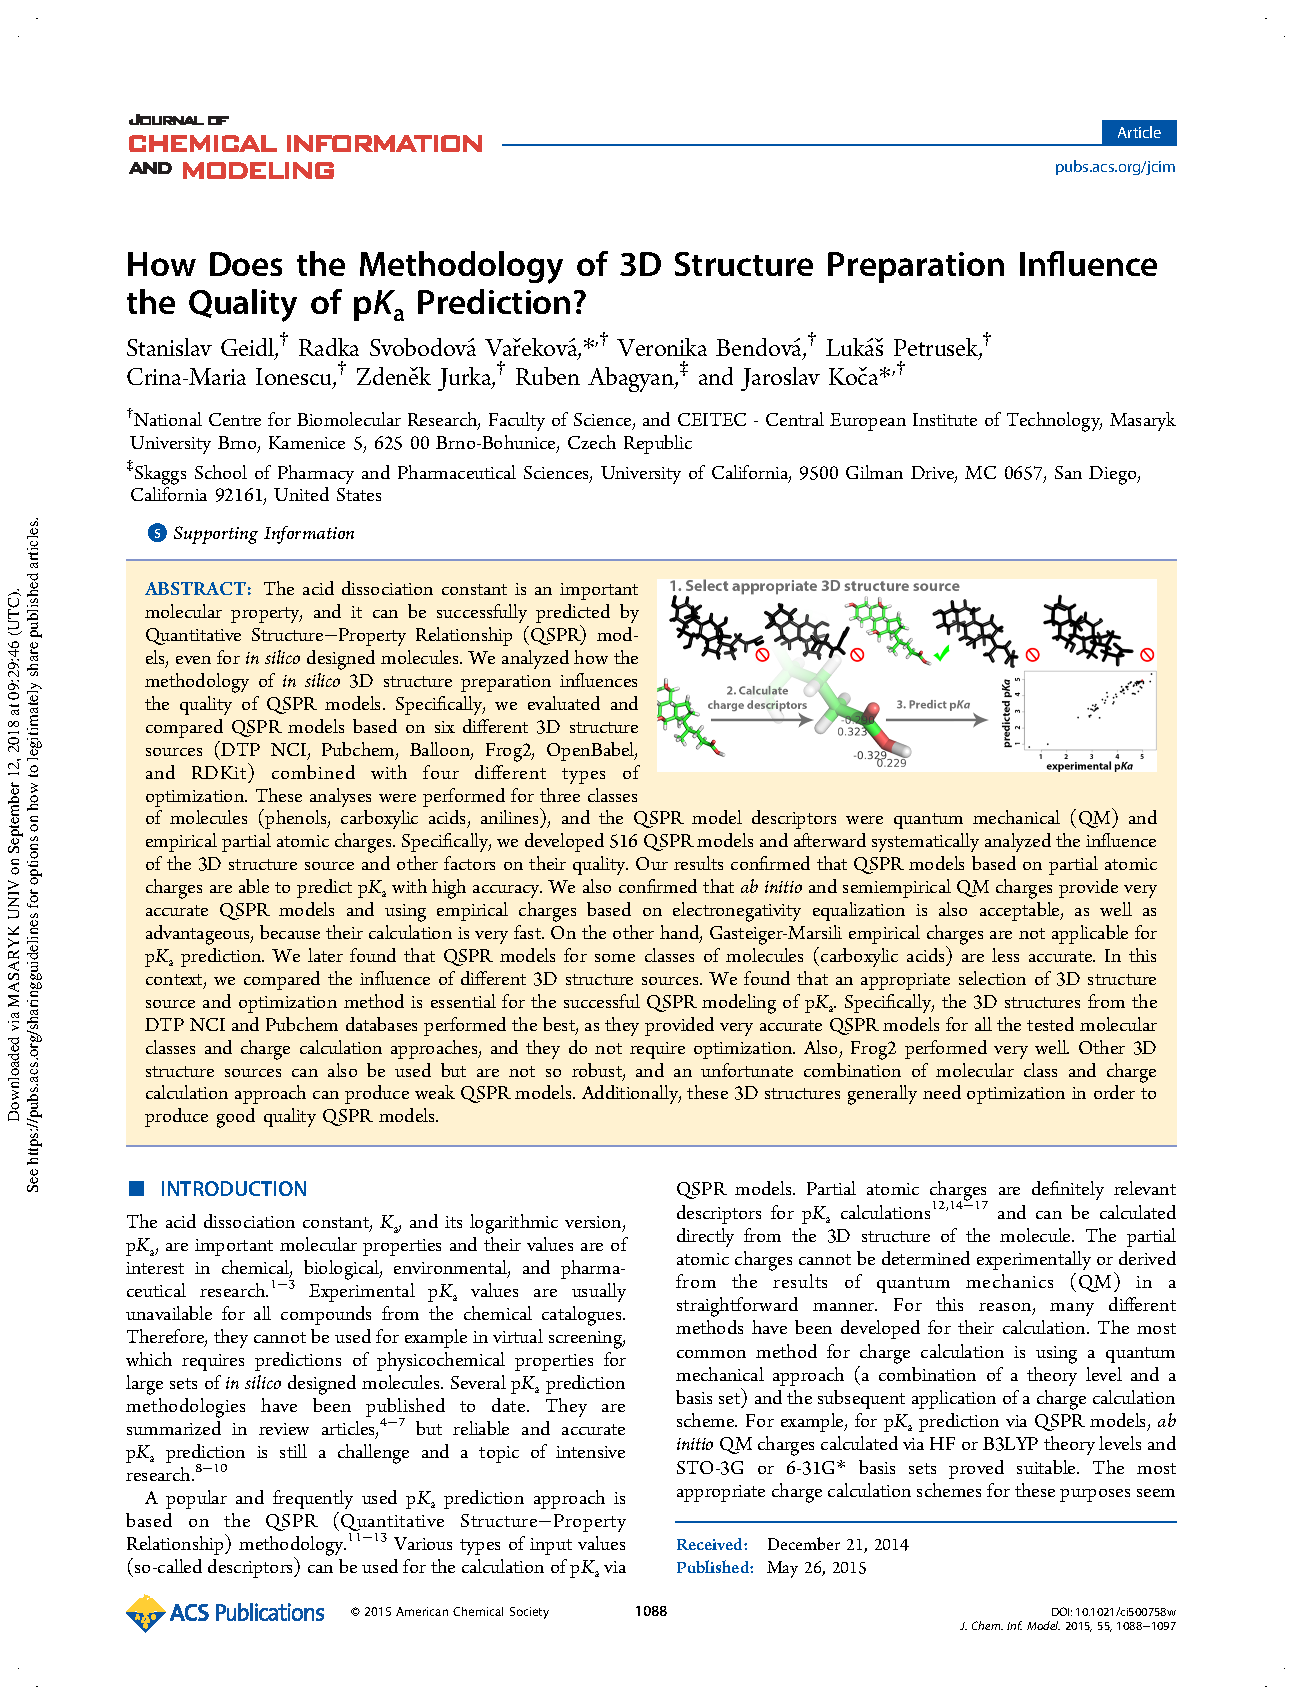
\includepdf[pages=-]{articles/pka.pdf}
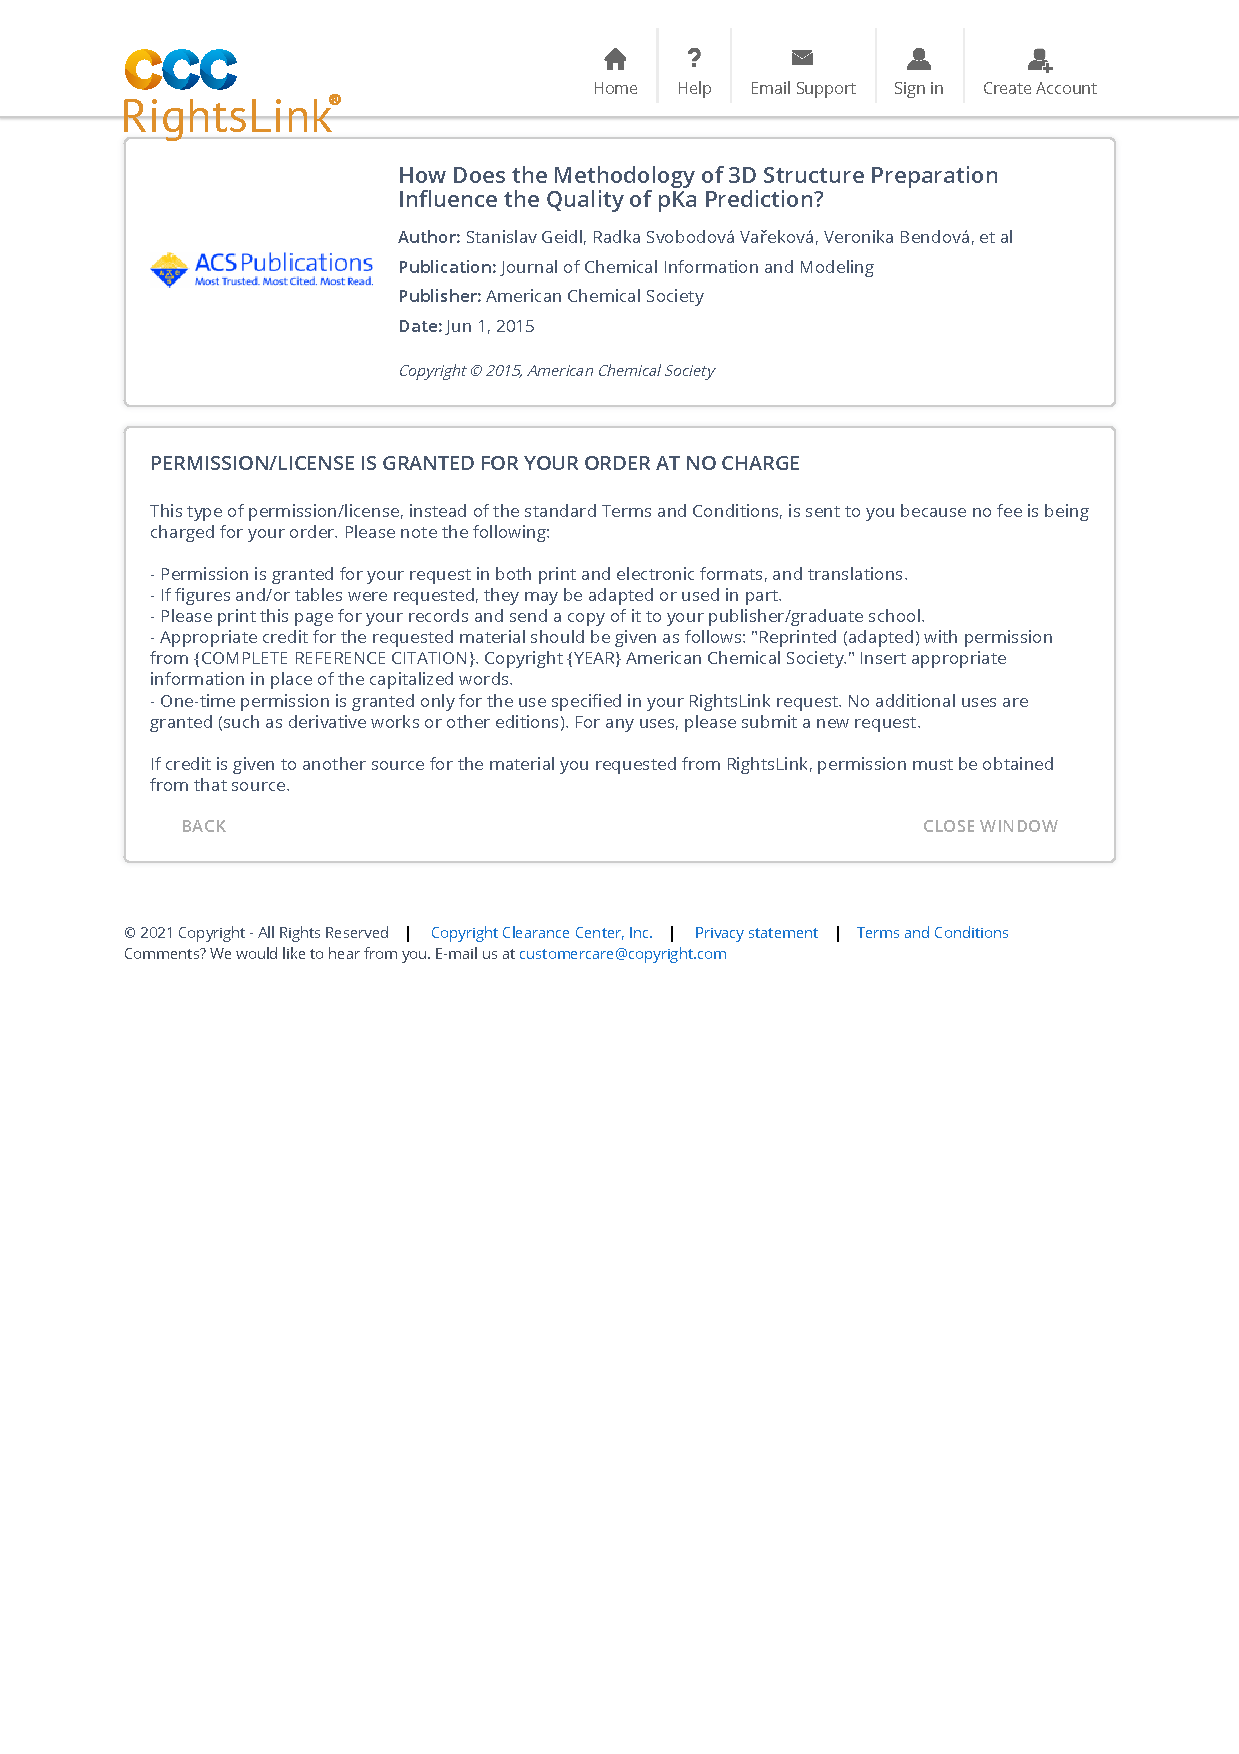
\includepdf[pages=-]{licenses/pka_license.pdf}


%%%

\begin{center}
\section{High-Quality and Universal Empirical Atomic
Charges for Chemoinformatics Applications}

\underline{Stanislav Geidl}$^1$, Tomáš Bouchal$^1$, Tomáš Raček$^{1,2}$,
Radka Svobodová Vařeková$^{1, *}$, Václav Hejret$^1$, Aleš Křenek$^3$,
Ruben Abagyan$^4$, Jaroslav Koča$^{1, *}$

\vspace{1cm}

$^1$ National Centre for Biomolecular Research, Faculty of Science and CEITEC,
Central European Institute of Technology, Masaryk University Brno, Kamenice 5,
625 00 Brno, Czech Republic.

$^2$ Faculty of Informatics, Masaryk University Brno, Botanická 68a, 602 00 Brno,
Czech Republic.

$^3$ Institute of Computer Science, Masaryk University Brno, Botanická 68a,
602 00 Brno, Czech Republic.

$^4$ Skaggs School of Pharmacy and Pharmaceutical Sciences, University of
California, 9500 Gilman Drive, San Diego, MC 0657, USA.

\vspace{1cm}

\textit{Journal of Cheminformatics} 2015, \textbf{7}:59.

\vspace{1cm}

\url{https://doi.org/10.1186/s13321-015-0107-1}

\end{center}

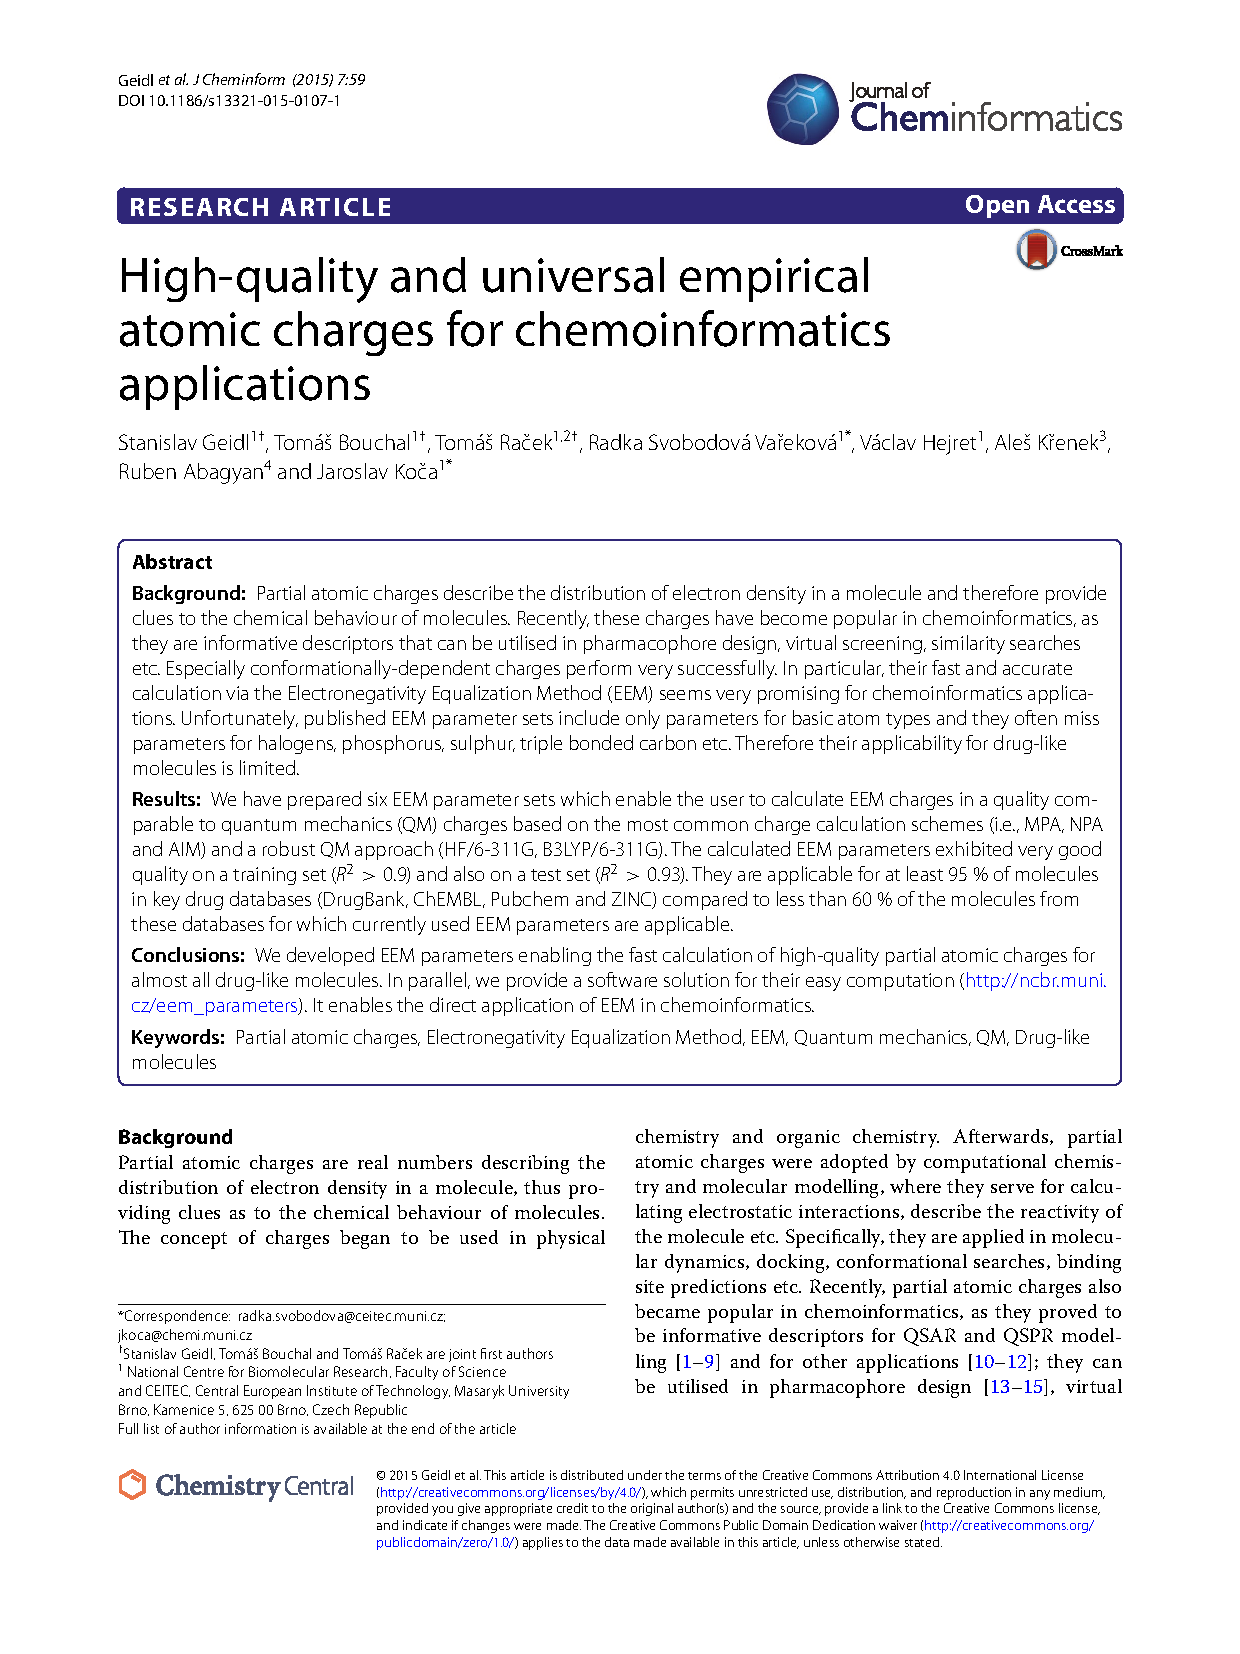
\includepdf[pages=-]{articles/eem.pdf}

%%%

\begin{center}

\section{NEEMP: Software
for Validation, Accurate Calculation and Fast Parameterization of EEM Charges}

Tomáš Raček$^{1,2,3}$, Jana Pazúriková$^{1,3}$, Radka Svobodová Vařekova$^{1,2,*}$,
\underline{Stanislav Geidl$^{1,2}$}, Aleš Křenek$^{1,2}$, Francesco Luca
Falginella$^1$, Vladimír Horský$^{1,3}$, Václav Hejret$^1$, Jaroslav Koča$^{1,2}$


\vspace{1cm}


$^1$ CEITEC -- Central European Institute of Technology,
Masaryk University Brno, Kamenice 5, 625 00 Brno, Czech Republic.

$^2$ National Centre for Biomolecular Research, Faculty of Science,
Masaryk University Brno, Kamenice 5, 625 00 Brno, Czech Republic.

$^3$ Faculty of Informatics, Masaryk University Brno, Botanická 68a, 602 00 Brno,
Czech Republic.

$^4$ Institute of Computer Science, Masaryk University Brno, Botanická 68a,
602 00 Brno, Czech Republic.

\vspace{1cm}

\textit{Journal of Cheminformatics} 2016, \textbf{8}:1

\vspace{1cm}

\url{https://doi.org/10.1186/s13321-016-0171-1}

\end{center}

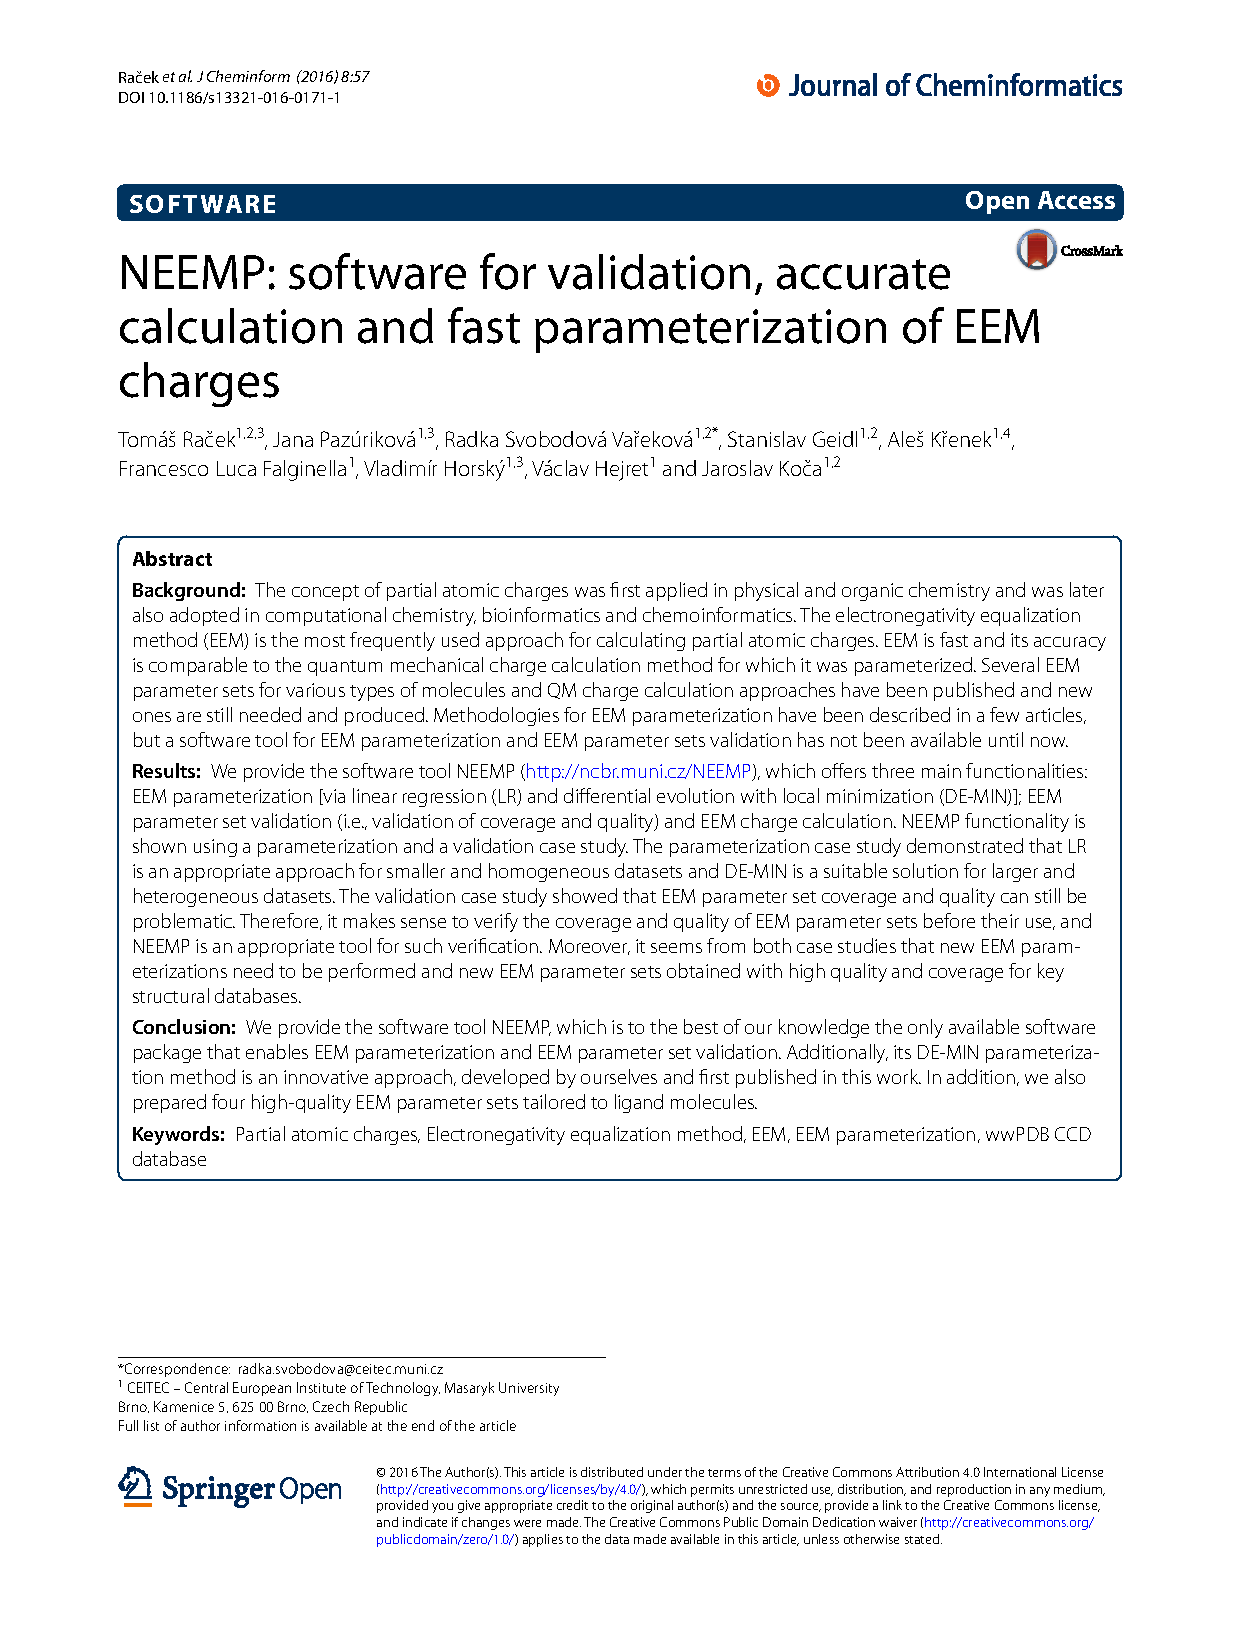
\includepdf[pages=-]{articles/neemp.pdf}
